% compilar con lualatex o xelatex
\documentclass[final]{beamer}

% poster de 90 x 140 cm en orientacion vertical
\usepackage[size=custom,width=90,height=140,scale=1.0]{beamerposter}

% idioma y tipografias
\usepackage[spanish, es-nodecimaldot]{babel}
%\usepackage{fontspec}
%\setsansfont{TeX Gyre Termes}
%\setmainfont{TeX Gyre Termes}

% paquetes utiles
\usepackage{booktabs}
\usepackage{multicol}
\usepackage{enumitem}
\usepackage{wrapfig}
\usepackage{tikz}
\usepackage{subcaption}
\usepackage{amsmath,amssymb,siunitx,graphicx,subcaption,booktabs,geometry,url,xcolor,tikz,caption}
\usepackage[percent]{overpic} % para superponer coordenadas en la imagen
\usepackage[spanish]{babel}
\usepackage{booktabs}   % Paquete para tablas
\usepackage{multirow}   % Para que el encabezado abarque dos filas
\usetikzlibrary{arrows.meta, positioning}
\usetikzlibrary{patterns}

% colores y estilo basico
\definecolor{azuludg}{RGB}{32,56,100}
\definecolor{azultext}{RGB}{47,85,151}
\definecolor{gris}{RGB}{80,80,80}
\setbeamercolor{headline}{fg=azuludg}
\setbeamercolor{title}{fg=azuludg}
\setbeamercolor{block title}{fg=white,bg=azuludg}
\setbeamercolor{block body}{fg=black,bg=white}

\captionsetup[table]{name=Tabla}
\renewcommand{\figurename}{Figura}
\setbeamertemplate{caption}[numbered]
\setbeamercolor{caption name}{fg=black}
\setbeamercolor{caption}{fg=black}

% separaciones de columnas y margenes internos
\setlength{\columnsep}{2.0cm}
\setlength{\columnseprule}{0pt}
\setbeamersize{text margin left=2.5cm,text margin right=2.5cm}

% encabezado del poster
\newcommand{\Header}{
  \begin{center}
    \begin{minipage}[c]{0.2\textwidth}
      
\includegraphics[height=8cm]{udg.pdf}
    \end{minipage} \hfill
    \begin{minipage}[c]{0.5\textwidth}
      \centering
      \Large \textbf{MAESTRÍA EN CIENCIAS EN INGENIERÍA ELÉCTRICA}\\
      \large \textbf{Difusión de Proyecto} \\
      \large \textbf{Guadalajara, Jalisco, Octubre 2025}
    \end{minipage} \hfill
    \begin{minipage}[c]{0.2\textwidth}
      \centering
      
\includegraphics[height=7.5cm]{cucei.pdf}
    \end{minipage}\par
    
    \vspace{1.2cm}
    {\Huge \textbf{\textcolor{azuludg}{Método Multivariable para la Identificación de Modos de Oscilación basado en el Algoritmo Tufts-Kumaresan.}} \par}
    \vspace{0.4cm}
    {\Large \textbf{\textcolor{azultext}{Ing. Glader David Hernández Reyes, Dr. Jose de Jesus Nuño Ayon}} \par}
  \end{center}
  \vspace{0.6cm}
  \noindent\rule{\textwidth}{4pt}
}




\begin{document}
\begin{frame}[t]
\Header

% bloque de resumen
\begin{block}{}
  \textbf{RESUMEN. }El monitoreo de la estabilidad en sistemas eléctricos de potencia 
  es crucial para garantizar una operación segura. Este proyecto se centra en el 
  desarrollo de un algoritmo Tufts-Kumaresan (TK) multivariable, diseñado para la 
  estimación robusta de modos de oscilación electromecánicos a partir de datos 
  sincrofasoriales (PMU). La metodología extiende la formulación clásica del TK para
   procesar simultáneamente múltiples señales, creando un sistema de predicción lineal 
   global que se resuelve mediante la Descomposición en Valores Singulares (SVD). 
   Este enfoque combina la alta robustez al ruido del algoritmo TK con la visión 
   sistémica del análisis multi-señal. Los resultados preliminares, validados con 
   señales sintéticas, demuestran que el método identifica correctamente los polos del 
   sistema y reconstruye las señales originales con alta fidelidad. El algoritmo 
   propuesto representa una herramienta prometedora para el diagnóstico preciso de la 
   estabilidad de pequeña señal en las complejas redes eléctricas modernas.\\
\vspace{32pt}
Palabras clave: \textbf{Análisis Modal, Tufts-Kumaresan, Estabilidad, Sistemas de Potencia, Modos Electromecánicos, WAMS, PMU, SVD, Procesamiento de Señales.}
\end{block}

% columnas principales
\begin{columns}[t,totalwidth=\textwidth]
  \begin{column}{0.49\textwidth}
    \begin{block}{\textbf{1. ANTECEDENTES Y JUSTIFICACIÓN}}
    La estabilidad de los sistemas eléctricos de potencia (SEP) es un pilar para la 
    operación confiable de la red \cite{ref1}. La llegada de los Sistemas de Medición 
    de Área Amplia (WAMS) ha revolucionado el monitoreo al proporcionar datos 
    sincrofasoriales (PMU) de alta resolución \cite{ref2}.
    \vspace{0.5cm}
  
    El algoritmo Tufts-Kumaresan (TK) mejora drásticamente la robustez al ruido 
    mediante la Descomposición en Valores Singulares (SVD) \cite{ref3}. Sin embargo, 
    su formulación original analiza una sola señal. Dado que los modos inter-área son 
    fenómenos globales, un enfoque multivariable es esencial para un análisis coherente
    \cite{ref4}. \textbf{Esta investigación se justifica por la necesidad de una 
    herramienta que combine la robustez del TK con la visión sistémica del análisis 
    multi-señal.}
    \end{block}

    \begin{block}{\textbf{2. DESCRIPCIÓN DEL PROBLEMA}}
    El problema central es la estimación precisa y robusta de los parámetros de los 
    modos de oscilación electromecánicos (frecuencia y amortiguamiento) a partir de 
    múltiples mediciones de PMUs. Se busca superar las limitaciones de los métodos de señal única, que pueden producir 
    resultados inconsistentes y dar información no deseada para la estabilidad del sistema.
    \end{block}

    \begin{block}{\textbf{3. OBJETIVO GENERAL E HIPÓTESIS}}
\textbf{Objetivo:} El desarrollo y la validación del algoritmo Tufts-Kumaresan multivariable 
para la estimación robusta y coherente de los modos electromecánicos en SEP, 
utilizando datos sincrofasoriales de PMUs.
    \vspace{0.5cm}
    
    \textbf{Hipótesis:} La implementación de un algoritmo TK multivariable permite 
    una reducción significativa en el error de estimación del factor de amortiguamiento
     en condiciones transitorias en la red, en comparación con el algoritmo TK de 
     una sola señal.
        \end{block}

    \begin{block}{\textbf{4. METODOLOGÍA}}
 El método propuesto sigue el flujo de proceso ilustrado en la Figura 
 \ref{fig:metodologia}. Se toman las mediciones de múltiples PMUs, se fusionan 
 en una matriz de predicción global y se aplica la SVD para aislar los modos 
 dominantes. Finalmente, se resuelve dos sistemas lineales: uno para 
 obtener los modos globales (frecuencia y amortiguamiento) y otro para determinar 
 la participación (amplitud y fase) de cada señal en dichos modos.
    
    \begin{figure}[h!]
        \centering
        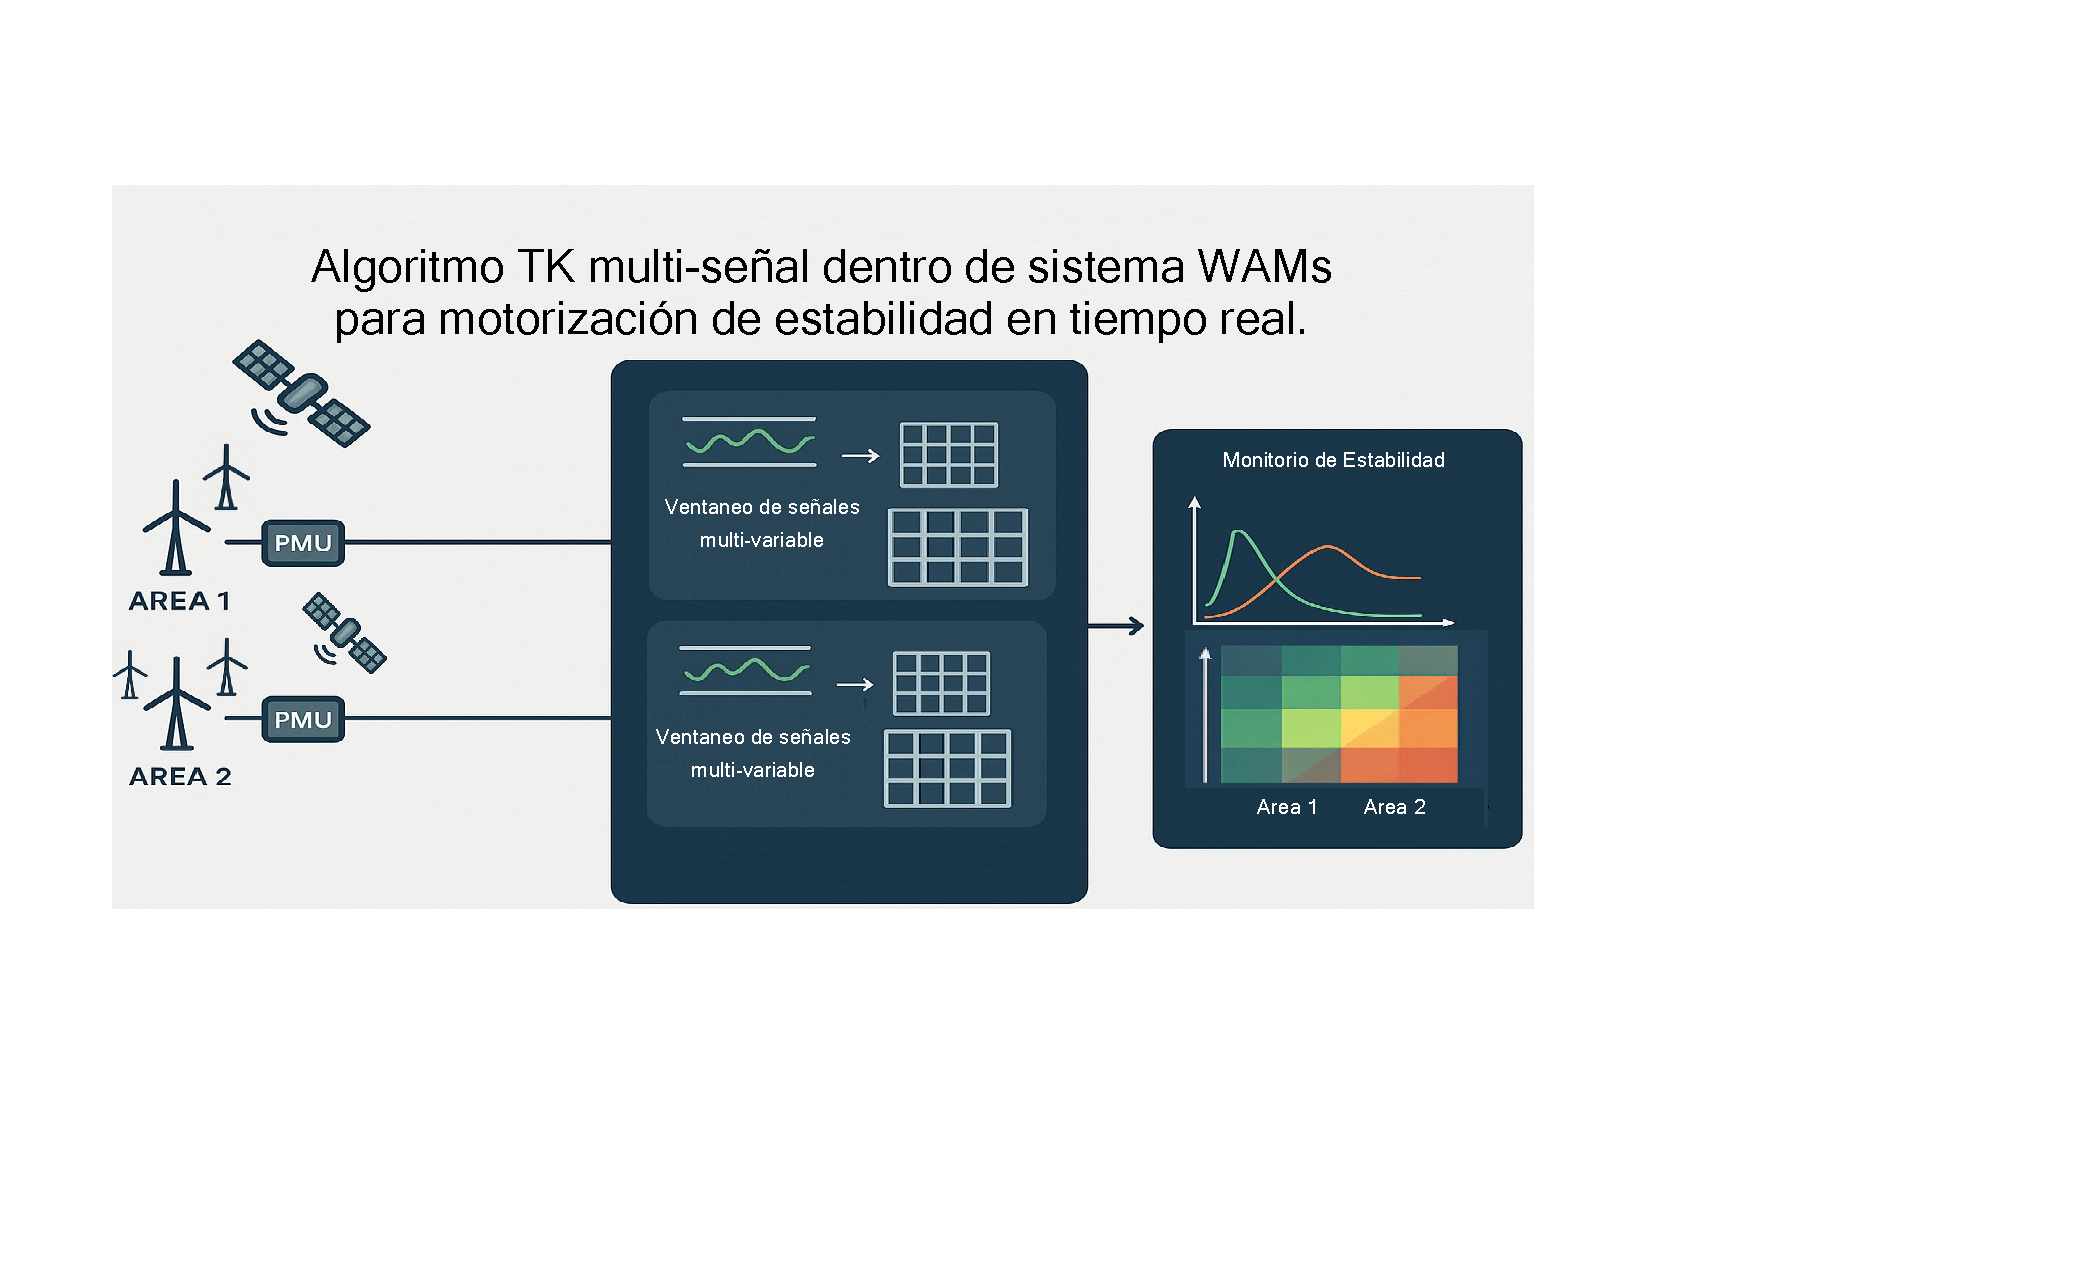
\includegraphics[width=0.5\columnwidth]{Metodologia.pdf}
        \caption{Diagrama de flujo del algoritmo Multi-TK propuesto.}
        \label{fig:metodologia}
    \end{figure}

\textbf{1. Adquisición y Modelado de Señales.}
    Se obtienen $P$ señales de velocidad angular de los generadores, muestreadas en 
    $N$ instantes de tiempo. Físicamente, cada señal $x_i[n]$ es una superposición 
    de $M$ modos de oscilación electromecánicos, los cuales se modelan matemáticamente
     como una suma de exponenciales complejas amortiguadas.
    
\begin{equation}
x_i[n] = \sum_{k=1}^{M} a_{i,k} e^{s_k n} + w_i[n], \quad 
\begin{cases}
n = 0,1,\ldots,N-1 \\
i = 1,2,\ldots,P
\end{cases}
\label{eq:signal_model}
\end{equation}

donde $a_{i,k} = |a_{i,k}| e^{j\phi_{i,k}}$ es la amplitud compleja del 
modo $k$ en la señal $i$, $s_k = -\delta_k + j\omega_k$ es el polo complejo del 
modo $k$, $\delta_k $ es el factor de amortiguamiento, $\omega_k$ es la frecuencia 
angular (rad/muestra) y $w_i[n]$ es ruido blanco gaussiano.

    \textbf{2. Ventaneo de Hankel.}
    Para extraer los parámetros modales de una señal, primero se estructura la 
    información en una matriz de predicción hacia atrás $\mathbf{A}_i$, comúnmente 
    conocida como matriz de Hankel. Esta matriz organiza las muestras de la señal de 
    tal manera que revela su dinámica interna.
    
\begin{equation}
\mathbf{A}_i = 
\begin{bmatrix}
x_i^*(1) & x_i^*(2) & \cdots & x_i^*(L) \\
x_i^*(2) & x_i^*(3) & \cdots & x_i^*(L+1) \\
\vdots & \vdots & \ddots & \vdots \\
x_i^*(N-L) & x_i^*(N-L+1) & \cdots & x_i^*(N-1)
\end{bmatrix}
\label{eq:A_matrix}
\end{equation}

    \textbf{3. Fusión de Datos y Expansión Multivariable.}
    Aquí reside la innovación clave. En lugar de analizar cada generador por separado,
     analizamos todos a la vez. Las matrices de Hankel $\mathbf{A}_i$ de cada una de 
     las $P$ señales se apilan verticalmente para formar una única matriz de 
     predicción global $\mathbf{A}_{\text{multi}}$. Esta matriz masiva captura las 
     dinámicas conjuntas de todo el sistema.
    \begin{equation}
        \mathbf{A}_{\text{multi}} = 
        \begin{bmatrix}
        \mathbf{A}_1^T & \mathbf{A}_2^T & \cdots & \mathbf{A}_P^T
        \end{bmatrix}^T
    \end{equation}
    
    \textbf{4. Filtrado con SVD.}
    La Descomposición en Valores Singulares (SVD) actúa como un filtro matemático avanzado. Al aplicarla a 
    $\mathbf{A}_{\text{multi}}$, podemos separar la información útil (los modos de oscilación
     coherentes) de modos no deseados. Nos quedamos solo con 
     los $M$ componentes más significativos para resolver el sistema de forma robusta.
    
La principal contribución de este trabajo es la combinación de múltiples señales 
para mejorar la robustez. Construimos el sistema global apilando verticalmente 
todas las matrices individuales:

\begin{equation}
\mathbf{A}_{\text{multi}} = 
\begin{bmatrix}
\mathbf{A}_1 \\
\mathbf{A}_2 \\
\vdots \\
\mathbf{A}_i
\end{bmatrix}, \quad
\mathbf{h}_{\text{multi}} = 
\begin{bmatrix}
\mathbf{h}_1 \\
\mathbf{h}_2 \\
\vdots \\
\mathbf{h}_i
\end{bmatrix}
\label{eq:multi_system}
\end{equation}

El sistema combinado resulta:

\begin{equation}
\mathbf{A}_{\text{multi}} \mathbf{b} = -\mathbf{h}_{\text{multi}}
\label{eq:multi_equation}
\end{equation}



El vector de coeficientes $\mathbf{b}$ se resuelve aplicando la SVD truncada a 
\eqref{eq:multi_equation}. Con $\mathbf{b}$ conocido, las raíces $z_k$ se obtienen
 del polinomio característico:


\begin{equation}
z^L + b(1)z^{L-1} + b(2)z^{L-2} + \cdots + b(L) = 0
\label{eq:characteristic_poly}
\end{equation}

Las raíces $z_k$ están relacionadas con los polos $s_k$ mediante 
$z_k = e^{s_k^*}$. A partir de estas raíces, se extraen los parámetros modales 
globales de amortiguamiento y frecuencia para cada modo $k$.


\begin{align}
\delta_k &= -\frac{1}{2\Delta t} \ln\left( [\text{Re}(z_k)]^2 + [\text{Im}(z_k)]^2 \right) \\
\omega_k &= \frac{1}{\Delta t} \arg(z_k)
\label{eq:frequency}
\end{align}

    \textbf{5. Estimación de Amplitudes con Matriz de Vandermonde.}
    Una vez que la SVD nos ha revelado los modos globales $z_k$ (frecuencia y 
    amortiguamiento), el problema de encontrar qué tanto participa cada generador 
    se vuelve lineal. Para cada señal $i$, se construye la matriz de Vandermonde 
    $\mathbf{\Psi}$ a partir de los modos $z_k$ conocidos:
    \begin{equation}
    \mathbf{\Psi} =
    \begin{bmatrix}
    z_1^0 & z_2^0 & \cdots & z_M^0 \\
    z_1^1 & z_2^1 & \cdots & z_M^1 \\
    \vdots & \vdots & \ddots & \vdots \\
    z_1^{N-1} & z_2^{N-1} & \cdots & z_M^{N-1}
    \end{bmatrix}
    \end{equation}
    Resolviendo el sistema $\mathbf{x}_i \approx \mathbf{\Psi} \mathbf{a}_i$, 
    obtenemos el vector $\mathbf{a}_i$, que contiene las amplitudes y desfases 
    específicos de cada modo para esa señal.
    

    \end{block}
  \end{column}

  \begin{column}{0.49\textwidth}
    \begin{block}{\textbf{5. RESULTADOS OBTENIDOS}}
    
  \textbf{Validación con Señales Sintéticas.} Se validó la precisión del algoritmo con un conjunto 
  de señales sintéticas compuestas por 4 modos oscilatorios. A continuación, se presenta la tabla 
  con los parámetros exactos de los cuatro modos de oscilación utilizados para generar las señales
  sintéticas.

\begin{table}[h!]
\centering
\caption{Parámetros de las señales sintéticas multicomponentes y valores estimados por el algoritmo TK.}
\label{tab:synthetic_signals}
\begin{tabular}{c c c c c c c c c c c}
\hline
\textbf{$x_i(t)$} & \textbf{$k$} & \textbf{$|a_{i,k}|$} & \textbf{$\delta_k$} & \textbf{$f_k$ (Hz)} & \textbf{$\phi_{i,k}$ (Grad)} & \textbf{$\lambda_k$ (TK)} & \textbf{$|a_{TK i,k}|$} & \textbf{$\delta_{TK i}$} & \textbf{$f_{TK i}$ (Hz)} & \textbf{$\phi_{TK i,k}$ (Grad)} \\
\hline
$x_1(t)$ & 1 & 1.00 & -0.050 & 0.60 & 0    & $-0.1885 + j3.7699$  & 1.00 & -0.0499 & 0.60 & 45.0 \\
         & 2 & 0.50 & -0.008 & 1.65 & 45   & $-0.0829 + j10.3673$ & 0.50 & -0.0080 & 1.65 & -90.0 \\
         & 3 & 0.20 & -0.030 & 0.95 & -90  & $-0.1791 + j5.9690$  & 0.20 & -0.0299 & 0.95 & -0.0 \\
         & 4 & 1.50 & -0.500 & 0.25 & 0    & $-0.7854 + j1.5708$  & 1.50 & -0.4472 & 0.25 & -0.0 \\[3pt]
$x_2(t)$ & 1 & 0.70 & -0.050 & 0.60 & 22.5 & $-0.1885 + j3.7699$  & 0.70 & -0.0499 & 0.60 & -0.0 \\
         & 2 & 1.20 & -0.008 & 1.65 & 0    & $-0.0829 + j10.3673$ & 1.20 & -0.0080 & 1.65 & 60.0 \\
         & 3 & 3.00 & -0.030 & 0.95 & 60   & $-0.1791 + j5.9690$  & 3.00 & -0.0299 & 0.95 & 22.5 \\
         & 4 & 1.15 & -0.500 & 0.25 & -30  & $-0.7854 + j1.5708$  & 1.15 & -0.4472 & 0.25 & -30.0 \\[3pt]
$x_3(t)$ & 1 & 0.85 & -0.050 & 0.60 & -45  & $-0.1885 + j3.7699$  & 0.85 & -0.0499 & 0.60 & 90.0 \\
         & 2 & 0.50 & -0.008 & 1.65 & 90   & $-0.0829 + j10.3673$ & 0.50 & -0.0080 & 1.65 & -0.0 \\
         & 3 & 0.20 & -0.030 & 0.95 & 0    & $-0.1791 + j5.9690$  & 0.20 & -0.0299 & 0.95 & -45.0 \\
         & 4 & 0.50 & -0.500 & 0.25 & 36   & $-0.7854 + j1.5708$  & 0.50 & -0.4472 & 0.25 & 36.0 \\[3pt]
$x_4(t)$ & 1 & 1.95 & -0.050 & 0.60 & 0    & $-0.1885 + j3.7699$  & 1.95 & -0.0499 & 0.60 & -60.0 \\
         & 2 & 0.75 & -0.008 & 1.65 & -60  & $-0.0829 + j10.3673$ & 0.75 & -0.0080 & 1.65 & -180.0 \\
         & 3 & 0.20 & -0.030 & 0.95 & 180  & $-0.1791 + j5.9690$  & 0.20 & -0.0299 & 0.95 & -0.0 \\
         & 4 & 1.25 & -0.500 & 0.25 & -90  & $-0.7854 + j1.5708$  & 1.25 & -0.4472 & 0.25 & -90.0 \\
\hline
\end{tabular}
\end{table}


    \begin{figure}[h!]
        \centering
        
\includegraphics[width=0.8\columnwidth]{Plano Z.pdf} % Usar \linewidth para que ocupe el ancho del minipage
        \caption{Identificación de polos en el plano Z.}
        \label{fig:plano_z}
    \end{figure}
 La Figura \ref{fig:plano_z} 
  confirma la correcta identificación de los polos del sistema fuera del círculo unitario.
    
    \begin{figure}[h!]
        \centering
        
\includegraphics[width=0.8\columnwidth]{Comparacion.pdf} % Usar \linewidth para que ocupe el ancho del minipage
        \caption{Comparación entre señales originales y reconstruidas.}
        \label{fig:comparacion}
    \end{figure}


  

La Figura \ref{fig:plano_z} muestra la identificación de polos en el plano Z, mientras que la Figura \ref{fig:comparacion} demuestra la alta fidelidad del método, donde las señales originales son reconstruidas casi a la perfección a partir de los parámetros modales estimados.
 

   \end{block}

    \begin{block}{\textbf{6. CONCLUSIONES Y TRABAJO FUTURO}}
    
       Se desarrolló y validó con éxito un algoritmo Tufts-Kumaresan multivariable.
       El método es capaz de identificar los modos globales a partir de señales sintéticas y de simulación con alta precisión.
       El enfoque Multi-TK se perfila como una técnica robusta y precisa para el análisis de estabilidad de pequeña señal.
    
    \vspace{0.5cm}
    \textbf{Trabajo Futuro:}
  
       Analizar las formas modales para determinar la participación de cada generador en los modos críticos.
       Cuantificar la robustez del algoritmo bajo diferentes niveles de ruido.
      Comparar su rendimiento con otras técnicas de la literatura.
   
    \end{block}

    \begin{block}{\textbf{REFERENCIAS}}
    % ejemplo de lista de referencias simple (puedes usar biblatex si prefieres)
    \begin{thebibliography}{9}\setlength{\itemsep}{2pt}
      \bibitem{ref1} P. Kundur, \emph{Power System Stability and Control}, 1st~ed. McGraw-Hill, 1994.
      \bibitem{ref2} P. W. Sauer, M. A. Pai, and J. H. Chow, \emph{Power System Dynamics and Stability with Synchrophasor Measurement}, 2nd~ed. Wiley-IEEE Press, 2018.
      \bibitem{ref3} R. Kumaresan and D. W. Tufts, "Estimating the parameters of exponentially damped sinusoids and pole-zero modeling in noise," \emph{IEEE Trans. Acoust., Speech, Signal Process.}, vol. 30, no. 6, pp. 833–840, Dec. 1982.
      \bibitem{ref4} C. A. Ordóñez and M. A. Ríos, "Electromechanical Modes Identification Based on Sliding-window Data from a Wide-area Monitoring System," \emph{Electr. Power Compon. Syst.}, vol. 41, no. 13, pp. 1264–1279, 2013.
    \end{thebibliography}
    \end{block}
  \end{column}
\end{columns}

\end{frame}
\end{document}
